\documentclass[10pt]{article}

\def\Type{LessonCaelan}
\def\TypeNum{Lesson 7}
\def\TypeTitle{Product \& Quotient Rules\\Notes To Instructors }
\def\Semester{Fall 2021} %Not Used 
\def\Course{MATH 1190 \& 1210}
\def\Targets{ {\bf\color{ForestGreen}D2} }

\usepackage{preambleDJ}




%%%%%%%%%%%% BEGIN DOCUMENT %%%%%%%%%%%%%%%
%%%%%%%%%%%% BEGIN DOCUMENT %%%%%%%%%%%%%%%
%%%%%%%%%%%% BEGIN DOCUMENT %%%%%%%%%%%%%%%
%%%%%%%%%%%% BEGIN DOCUMENT %%%%%%%%%%%%%%%
%%%%%%%%%%%% BEGIN DOCUMENT %%%%%%%%%%%%%%%



\begin{document}

\pagestyle{otherpages}
\thispagestyle{firstpage}
\vs{.6}

\lt  
\enumC{
\item[\target{D2}:] Compute Derivatives
\itemC{
 \item Apply the product rule and the quotient rule to take the derivative. 
}
}



\lg Students will be able to...
\enumCN{
\item Find the derivative using the product rule, the quotient rule, and possibly a combination of them.
}

\feed
\itemC{
\item Most students found the pre-class clear
\item Students commented on how product and quotient rules are different from the power rule. They said they would appreciate more practice.
}

 \hand
 \itemI{
 \item {\bf Warm-up Exercise $1$} is designed to give students practice with exponent rules $x^{a/b} = \sqrt[b]{x^a}$ and $x^{-n} = \dfrac{1}{x^n}$
 \item {\bf Warm-up Exercise $2$} asks students to regurgitate differentiation rules learned in pre-class activity.
 \item {\bf Exercise A} provides practice with basic differentiation rules and  some use of exponent rules and other algebra. In particular, problem k) is on worksheet to address students question.
 \item {\bf Exercise B} Provides practice finding derivatives, understanding how to interpret the meaning of a derivative and apply these ideas in context of a multi-step problem.
 \item {\bf Extra Practice $1$ and $2$} give more practice contextualizing derivatives. 
 }

\core Exercise B, extra practice 1

\newpage

\textbf{Intended Learning Outcomes}
After this lesson, you will be able to 

\begin{itemize}
    \item Apply the product rule and the quotient rule to take the derivative. (\target{D2})
\end{itemize}

\vspace{-0.5cm}

\hrulefill

\paragraph*{GOAL:} The goal of this lesson is for you to become fluent in applying the product \& quotient rules in a variety of contexts.\\

{\bf\color{blue}Warm-up Exercise 1.} Please complete the Product Rule: $\displaystyle \frac{d}{dx}[f(x)g(x)]=$ \blue{$f'(x)g(x)+f(x)g'(x)$}  

{\example{\bf\color{ForestGreen}D2}} Find the following derivative:\\

$\dfrac{d}{dx}\left[(1-\sqrt[3]{x})(x^2-8x)\right]\bigg|_{x=8}$\\

$\blue{\dfrac{d}{dx}\left[(1-\sqrt[3]{x})(x^2-8x)\right]=-\dfrac{1}{3}x^{-2/3}(x^2-8x)+(2x-8)(1-\sqrt[3]{x})}$

\blue{Plug in $x=8$, we get $-\dfrac{1}{3}8^{-2/3}(8^2-8(8))+(2(8)-8)(1-\sqrt[3]{8})=-8$}

\vfill

{\exercise{\bf\color{ForestGreen}D2}} Find the following derivatives:\\

\begin{enumerate}
\item[(a)] $\dfrac{d}{dx}[(x^2+x+1)(4-2x)]=\blue{(2x+1)(4-2x)-2(x^2+x+1)}$

\vfill

\item[(b)] $\dfrac{d}{dx}[(x^3-2x^2)(\sqrt{x}+4)]\bigg|_{x=1}$

$\blue{\dfrac{d}{dx}\left[(x^3-2x^2)(\sqrt{x}+4)\right]=(3x^2-4x)(\sqrt{x}+4)+\dfrac{1}{2\sqrt{x}}(x^2-2x^2)}$

\blue{Plug in $x=1$, we get $(3(1)^2-4(1))(\sqrt{1}+4)+\dfrac{1}{2\sqrt{1}}((1)^3-2(1)^2)=-\dfrac{11}{2}$}

\vfill
\vfill

\item[(c)] $\dfrac{d}{dt}\left[ t\cdot f(t) \right]\bigg|_{t=2}$, where $f(2)=-3$ and $f'(2)=7$

$\blue{\dfrac{d}{dt}\left[ t\cdot f(t) \right]=f(t)+t\cdot f'(t)}$

\blue{Plug in $t=2$, we get $-3+2\cdot 7=11$}

\vfill
\vfill

\end{enumerate}

\newpage

{\bf\color{blue}Warm-up Exercise 2.} Please complete the Quotient Rule: $\dfrac{d}{dx}\left[ \dfrac{hi(x)}{lo(x)} \right] =\blue{\dfrac{lo(x)hi'(x)-hi(x)lo'(x)}{(lo(x))^2}}$ \\

{\example{\bf\color{ForestGreen}D2}} Find the following derivative:\\

$\dfrac{d}{dy}\left[ \dfrac{y^3-y^2+1}{1-y} \right]\bigg|_{y=0}$

\blue{

$\dfrac{d}{dy}\left[ \dfrac{y^3-y^2+1}{1-y}\right] = \dfrac{(1-y)(3y^2-2y)-(y^3-y^2+1)(-1)}{(1-y)^2}$

Plug in $y=0$, we get $\dfrac{(1-0)(3(0)^2-2(0))-((0)^3-(0)^2+1)(-1)}{(1-0)^2}=1$

}

\vfill

{\exercise{\bf\color{ForestGreen}D2}} Find the following derivatives:\\

\begin{enumerate}
\item[(a)] $\dfrac{d}{dt}\left[ \dfrac{f(t)}{g(t)} \right]\bigg|_{t=1}$, where $f(1)=2$, $f'(1)=3$, $g(1)=-3$, and $g'(1)=-1$

\blue{$\dfrac{d}{dt}\left[ \dfrac{f(t)}{g(t)} \right]\bigg|_{t=1}=\dfrac{f'(t)g(t)-f(t)g'(t)}{(g(t))^2}\bigg|_{t=1}=\dfrac{f'(1)g(1)-f(1)g'(1)}{(g(1))^2}=-\dfrac{7}{9}$}

\vfill

\item[(b)] $\dfrac{d}{dz}\left[ \dfrac{z^3}{1+z^2} \right]$

\blue{$\dfrac{d}{dz}\left[ \dfrac{z^3}{1+z^2} \right]=\dfrac{3z^2(1+z^2)-z^3(2z)}{(1+z^2)^2}$}

\vfill

%%%%%%%%% 
\newpage%
%%%%%%%%%

\item[(c)] $\dfrac{d}{dz}\left[ \dfrac{z^3g(z)}{1+z^2} \right]\bigg|_{z=1}$, where $g(1)=0$ and $g'(1)=-2$

\blue{$\dfrac{d}{dz}\left[ \dfrac{z^3g(z)}{1+z^2} \right]\bigg|_{z=1}=\dfrac{(3z^2g(z)+z^3g'(z))(1+z^2)-z^3g(z)(2z)}{(1+z^2)^2}\bigg|_{z=1}\\\\=\dfrac{(3(1)^2g(1)+(1)^3g'(1))(1+(1)^2)-(1)^3g(1)(2)}{(1+(1)^2)^2}=\dfrac{-4-0}{4}=-1$}

\vfill
\vfill

\item[(d)] $\dfrac{d}{dt}\left[ \dfrac{\sqrt[3]{t}+1}{e^t(t^2-2t+2)} \right]$

\blue{

$\dfrac{d}{dt}\left[ \dfrac{\sqrt[3]{t}+1}{e^t(t^2-2t+2)} \right]=\dfrac{(1/3)t^{-2/3}e^t(t^2-2t+2)-(\sqrt[3]{t}+1)(e^t(t^2-2t+2)+e^t(2t-2)}{e^{2t}(t^2-2t+2)^2}$

}

\vfill
\vfill
\vfill

\end{enumerate}

{\bf REVIEW:} How do we interpret the derivative of a function geometrically? This exercise will give you an opportunity to refresh your memory on this critical property.

\begin{minipage}[t]{0.55\textwidth}
{\bf\color{blue} Extra Practice 1.} %\reversemarginpar\marginnote{\fbox{\bf\color{ForestGreen}D2}} 
Let $p(x)=f(x)g(x)$ and let $q(x)=\dfrac{f(x)}{g(x)}$, where $f$ and $g$ are functions whose graphs are shown to the right. What are the values of $p'(1)$ \& $q'(5)$? \\
\end{minipage}
\hfill
\begin{minipage}[t]{0.4\textwidth}
\,
\begin{center}
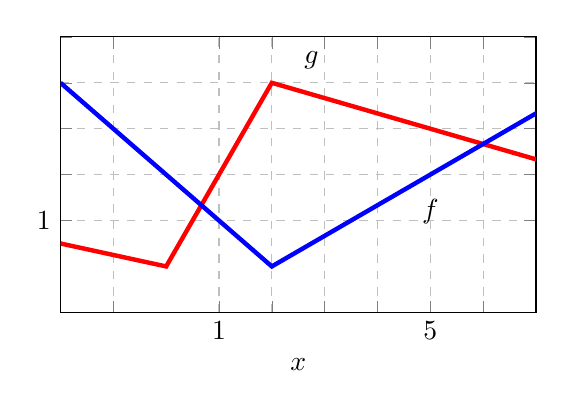
\begin{tikzpicture}
  \begin{axis}[
    xlabel={$x$},
    xtick       = {-2,-1,1,2,3,4,5,6,7},
    xticklabels = { , ,$1$, , , ,$5$ , , },
    ytick       = {-1,1,2,3,4,5},
    yticklabels = { ,$1$, , , , },
    samples     = 320,
    domain      = -3.5:3.5,
    %restrict y to domain=-2.5:4.5,
    xmin = -2, xmax = 7,
    ymin = -1, ymax = 5,
    width = 3in, height = 2in,
    grid=both, grid style=dashed
  ]
  \draw[red,ultra thick] (-2,0.5) -- (0,0) -- (2,4) -- (8,2);
  \node at (2.75,4.5) {$g$};
  \draw[blue,ultra thick] (-2,4) -- (2,0) -- (8,4);
  \node at (5,1.2) {$f$};
\end{axis}
\end{tikzpicture}
\end{center}
\end{minipage}

\blue{

$p'(x)=f'(x)g(x)+f(x)g'(x)$

Plug in $x=1$ gives $p'(1)=f'(1)g(1)+f(1)g'(1)=(-1)(2)+(1)(2)=0$.

$q'(x)=\dfrac{f'(x)g(x)-f(x)g'(x)}{(g(x))^2}$

Plug in $x=5$ gives $\dfrac{f'(5)g(5)-f(5)g'(5)}{(g(5))^2}=\dfrac{(2/3)(3)-(2)(-1/3)}{(3)^2}=\dfrac{8}{27}$

}

\vfill

%%%%%%%%%
\newpage%
%%%%%%%%%

{\bf REVIEW:} How do we interpret the derivative of a function when that function represents a known quantity? The next two exercises will give you an opportunity to keep the answer to that question fresh in your mind as you practice using relevant differentiation rules!\\

{\bf\color{blue}Extra Practice 2.} %\reversemarginpar\marginnote{\fbox{\bf\color{ForestGreen}D2}} 
Kinesiologists track sprinters' heart rates after completing a $400$ meter sprint to get a better sense of strain on athletes' cardiovascular systems after an intense workout. Collected data suggest that the function $f(t)=\dfrac{120}{1+\sqrt{t}}$ can be used to predict how elevated a sprinter's heart rate (in $\frac{\text{beats}}{\text{minute}}$) will be above their resting heart rate $t$ minutes after completing the $400$ meter sprint.


\begin{enumerate}
%\item[i.] How elevated does the model predict a sprinter's heart rate will be immediately after completing the $400$ meter sprint? Include units of measurement in your answer.

%\vfill

\item[(a)] Find $f'(4)$. 

\blue{

$f'(t)=\dfrac{-120(1/2)t^{-1/2}}{(1+\sqrt{t})^2}=\dfrac{-60t^{-1/2}}{(1+\sqrt{t})^2}$

$f'(4)=\dfrac{-60(4)^{-1/2}}{(1+\sqrt{4})^2}=\dfrac{-60(1/2)}{9}=-\dfrac{10}{3}$

}

\vfill
\vfill

\item[(b)] What are the units of measurement of $f'(4)$? \blue{$\frac{\text{beats}}{\text{minute}^2}$}

\item[(c)] What does $f'(4)$ represent in this context? ({\bf Note:} ``in this context" means your answer must clearly relate to the scenario described in the problem. Answers like ``the derivative of $f$ when $t=4$" are not in context.)

\blue{At 4 minutes after completing the 400 meter sprint, if another minute passes by, the sprinter's heart rate would change by approximately $f'(4)$ $\frac{\text{beats}}{\text{minute}}$.}

\vfill

\item[(d)] Below are graphs of $f$, $f'$, and $f''$ considered in this problem together on the same coordinate grid. Which of the following is the correct assignment? Select one:\\

\begin{minipage}[t][3.25in][t]{.3\textwidth}
\enumA{
    \item $\begin{cases}\text{solid:} & f'' \\\text{dashed:} & f' \\\text{dotted:} & f \end{cases}$
    \item $\begin{cases}\text{solid:} & f'' \\\text{dashed:} & f \\\text{dotted:} & f' \end{cases}$
    \item $\begin{cases}\text{solid:} & f'\\\text{dashed:} & f'' \\\text{dotted:} & f \end{cases}$
    \item $\begin{cases}\text{solid:} & f\\\text{dashed:} & f''\\\text{dotted:} & f' \end{cases}$
    \item none of the above
}
\end{minipage}
%
\hfill
%
\begin{minipage}[t][3.25in][t]{.68\textwidth}
\,

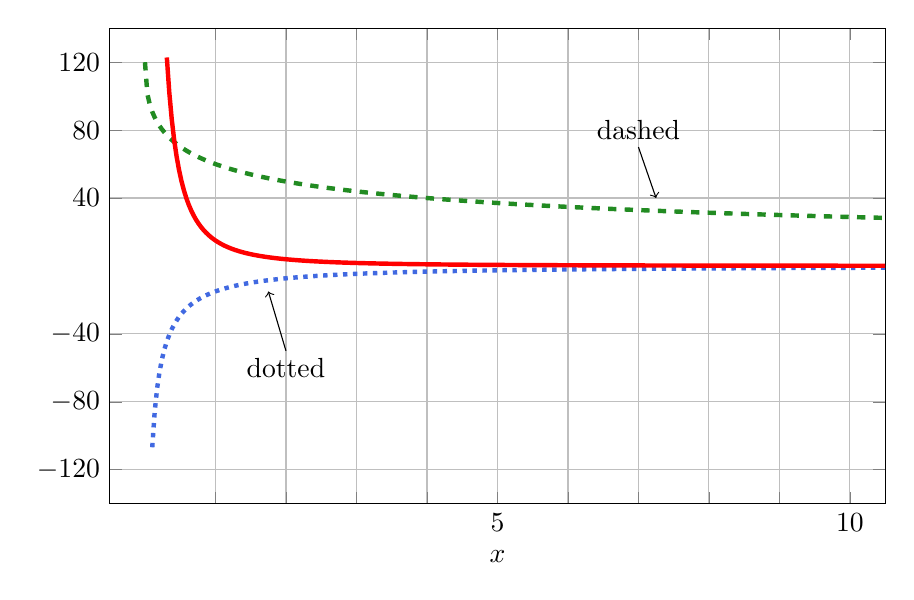
\begin{tikzpicture}
    \begin{axis}[
            xlabel={$x$},
            xtick       = {1,2,3,4,5,6,7,8,9,10},
            xticklabels = {\,,\,,\,,\,,$5$,\,,\,,\,,\,,$10$},
            ytick       = {-120,-80,-40,40,80,120},
            yticklabels = {$-120$,$-80$,$-40$,$40$,$80$,$120$},
            samples     = 320,
            domain      = 0:11,
            restrict y to domain=-140:140,
            xmin = -0.5, xmax = 10.5,
            ymin = -140, ymax = 140,
            width=4.5in, height=3in,
            grid=both, grid style=solid
          ]
    % f
    \addplot[domain=0:11, ForestGreen, dashed, ultra thick, mark=none]{120/(1+x^(1/2))};
    % f'
    \addplot[domain=0:11, RoyalBlue, dotted, ultra thick, mark=none]{-60/(x^(3/2)+2*x+x^(1/2))};
    \node at (2,-60) {dotted};
    \draw[->] (2,-50) -- (1.75,-15);
    % f''
    \addplot[domain=0:11, Red, ultra thick, mark=none]{(30*x^(-3/2)*(1+x^(1/2))+60*x^(-1))/(1+x^(1/2))^3};
    \node at (7,80) {dashed};
    \draw[->] (7,70) -- (7.25,40);
    \end{axis}
\end{tikzpicture}

\end{minipage}

\end{enumerate}

\blue{(b) Try plug $t=0$ into $f(t)$.}
\end{document}
